%Also, for most of 5.2, you need to make the case that the single result you show 
%is representative!!  I think that's easy, but needs to be done.  Essentially, 
%you need to make the case that for real isotopes, the same model will be 
%invoked with real parameters, so that these normalized (relative?) parameters 
%are representative of all cases.
In the following base cases, basic transport behavior for aphysical 
parameterizations demonstrate the successful collective behavior of the modular 
components in a \Cyder repository.

\subsection{Basic Transport and Containment Problem Specification}

Basic transport and containment base cases were conducted to verify the 
fundamental behavior of all the radionuclide transport models at each component 
interface. These integration tests neglected thermal transport and capacity 
estimation to simplify the results.

The problem design includes the following : 
\begin{itemize}
\item{A source facility providing one waste stream per time step}
\item{An initial capacity of five 1 kg waste streams (in most cases)}
\item{Waste form Components each accepting 1 waste stream} 
\item{Corresponding waste package Components, one per waste form}
\item{A buffer Component}
\item{A far field Component}
\end{itemize}

This simulation is run for 1000 years.

\subsubsection{Mixed Cell Model}
The Mixed Cell model behaves similarly to the Degradation Rate model when 
sorption and solubility limitation in that model are disabled. When they are 
enabled, however, the system is expected to demonstrate sorption limited and 
solubility limited transport as in Figures \ref{fig:mcIIIall} through 
\ref{fig:mcII}. The extent to which sorption and solubility limitation meet 
expectations is addressed in this base case.


\begin{figure}[ht]
\centering
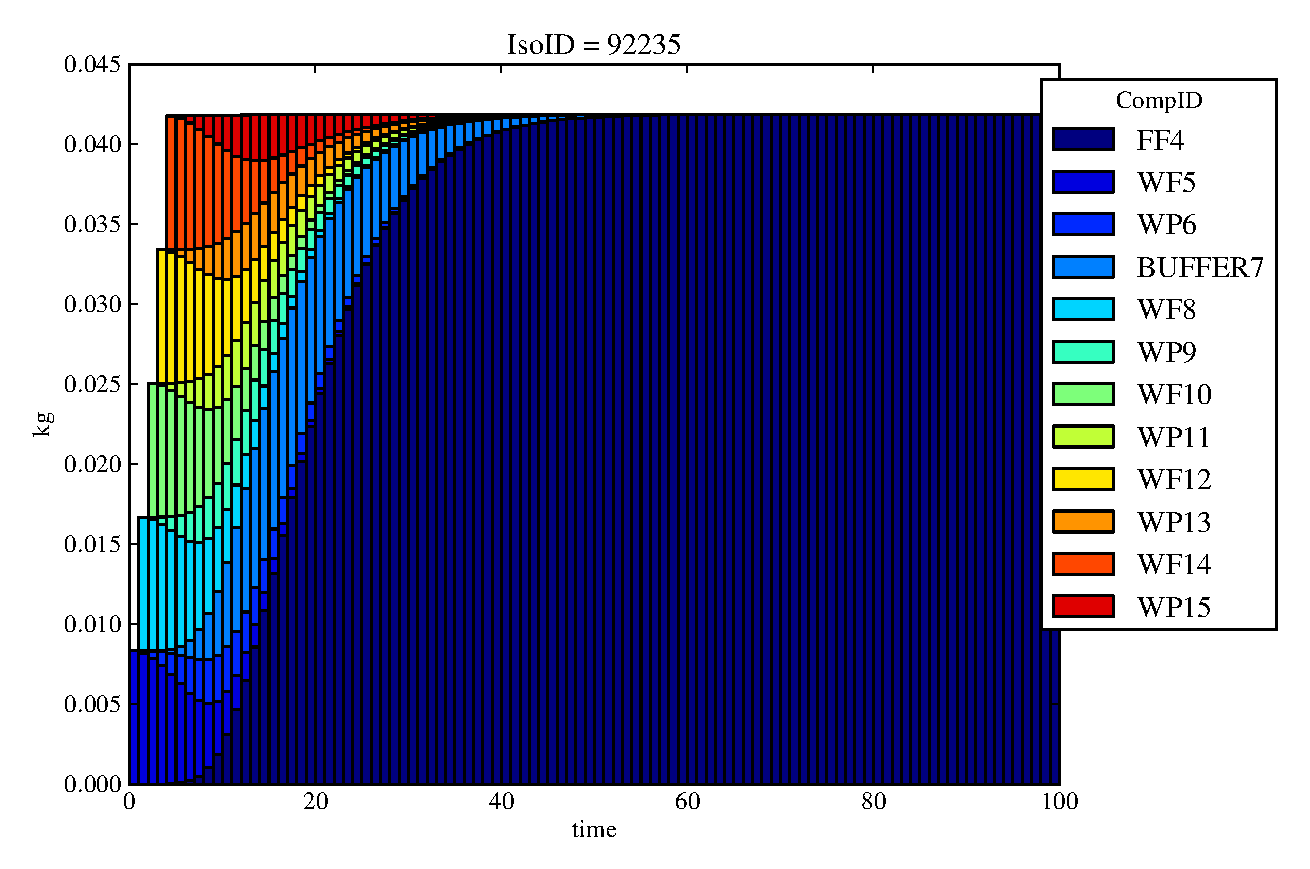
\includegraphics[width=0.6\textwidth]{./results/images/mcIII.eps}
\caption[$^{235}U$ residence. Mixed Cell Coupled Sorption and Solubility Limitation.]{
For the MCIII case in which containment is affected by solubility limitation,
        ($F_{d}=0.1$ for all components except far field), $^{235}U$ travels through waste 
        packages (WPN), their corresponding waste forms (WFN), and the surrounding 
        buffer (BUFFER7) more slowly than in the MCI case
        before permanent residence in the far field component (FF).
}
\label{fig:mcIIIall}
\end{figure}

\begin{figure}[ht]
\centering
  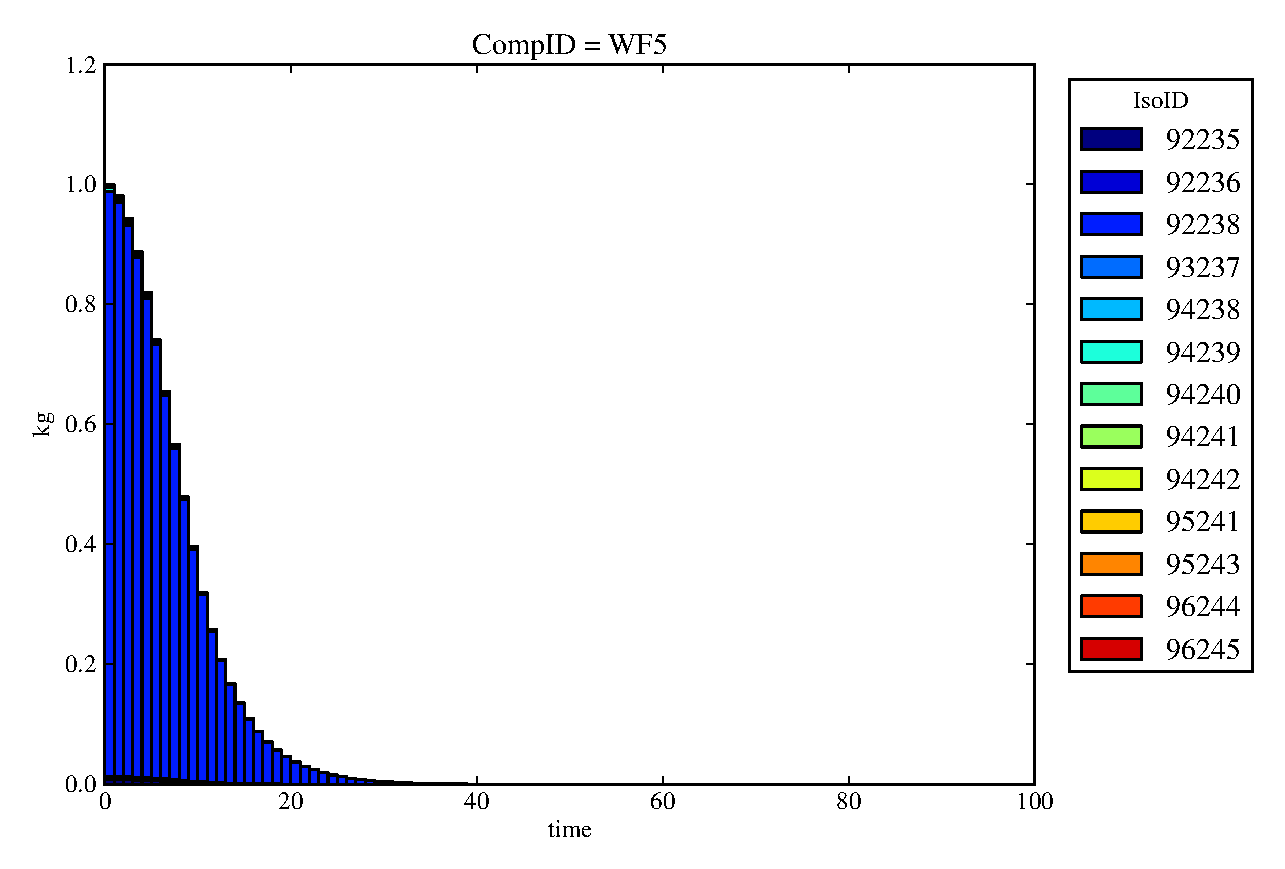
\includegraphics[width=0.6\textwidth]{./results/images/mcIII1.eps}
  \caption[Case MCIII Waste Form Contaminants.]{
          Waste Form 5 (degradation rate $F_d = 0.1[y^{-1}]$, reference solubility limit $S_{ref} = 0.001kg/m^3$) releases material with degradation.
    }
  \label{fig:mcIIIwf5}
\end{figure}


\begin{figure}[ht]
\centering
  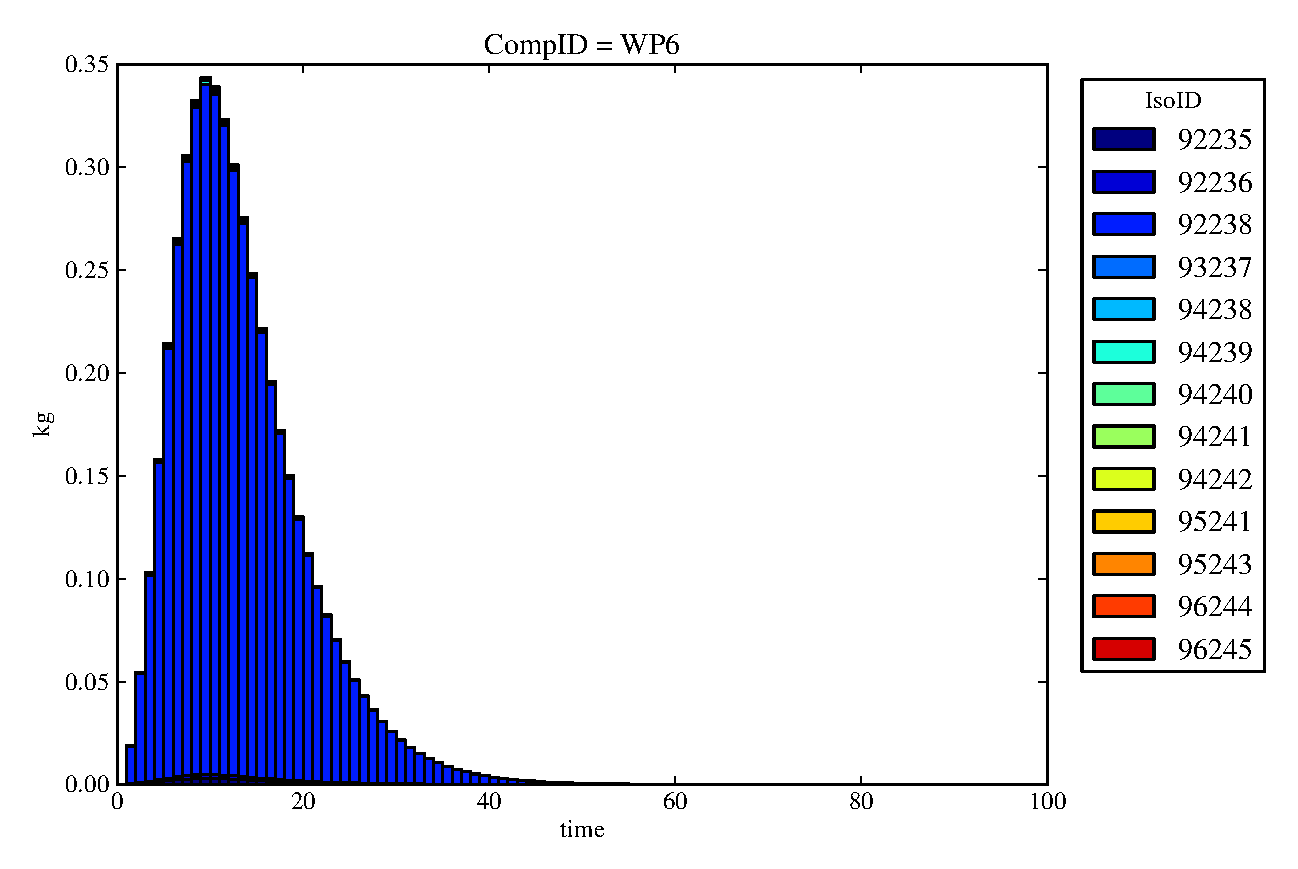
\includegraphics[width=0.6\textwidth]{./results/images/mcIII2.eps}
  \caption[Case MCIII Waste Package Contaminants.]{
          Waste Package 6 (degradation rate $F_d = 0.1[y^{-1}]$, reference solubility limit $S_{ref}=0.001kg/m^3$) receives then releases material.
    }
  \label{fig:mcIIIwp6}
\end{figure}

\begin{figure}[ht]
\centering
  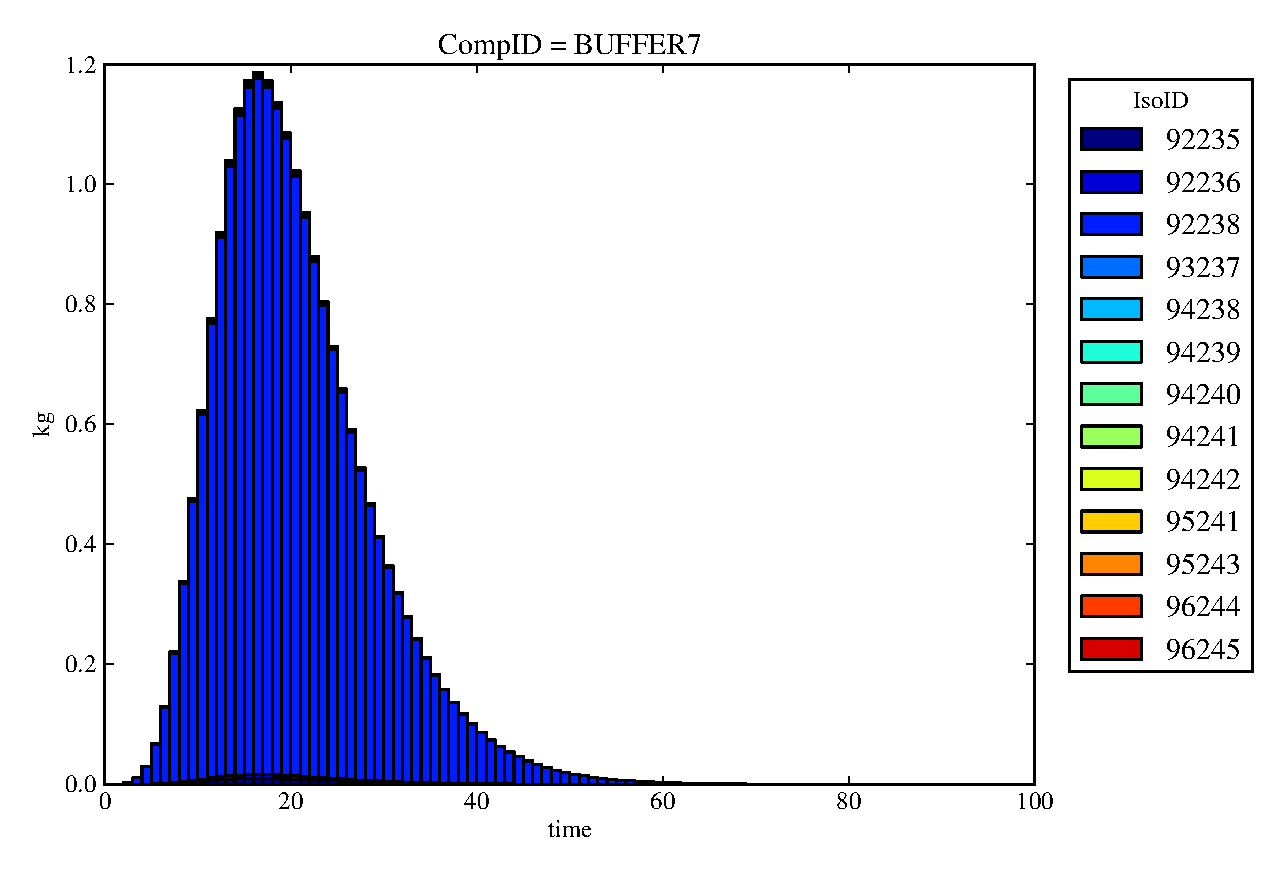
\includegraphics[width=0.6\textwidth]{./results/images/mcIII3.eps}
  \caption[Case MCIII Buffer Contaminants]{
          The Buffer, component 7 (degradation rate $F_d=0.1[y^{-1}]$, reference solubility 
        limit $S_{ref}=0.001kg/m^3$), receives and then releases material.
    }
  \label{fig:mcIIIbuff}
\end{figure}

\begin{figure}[ht]
\centering
  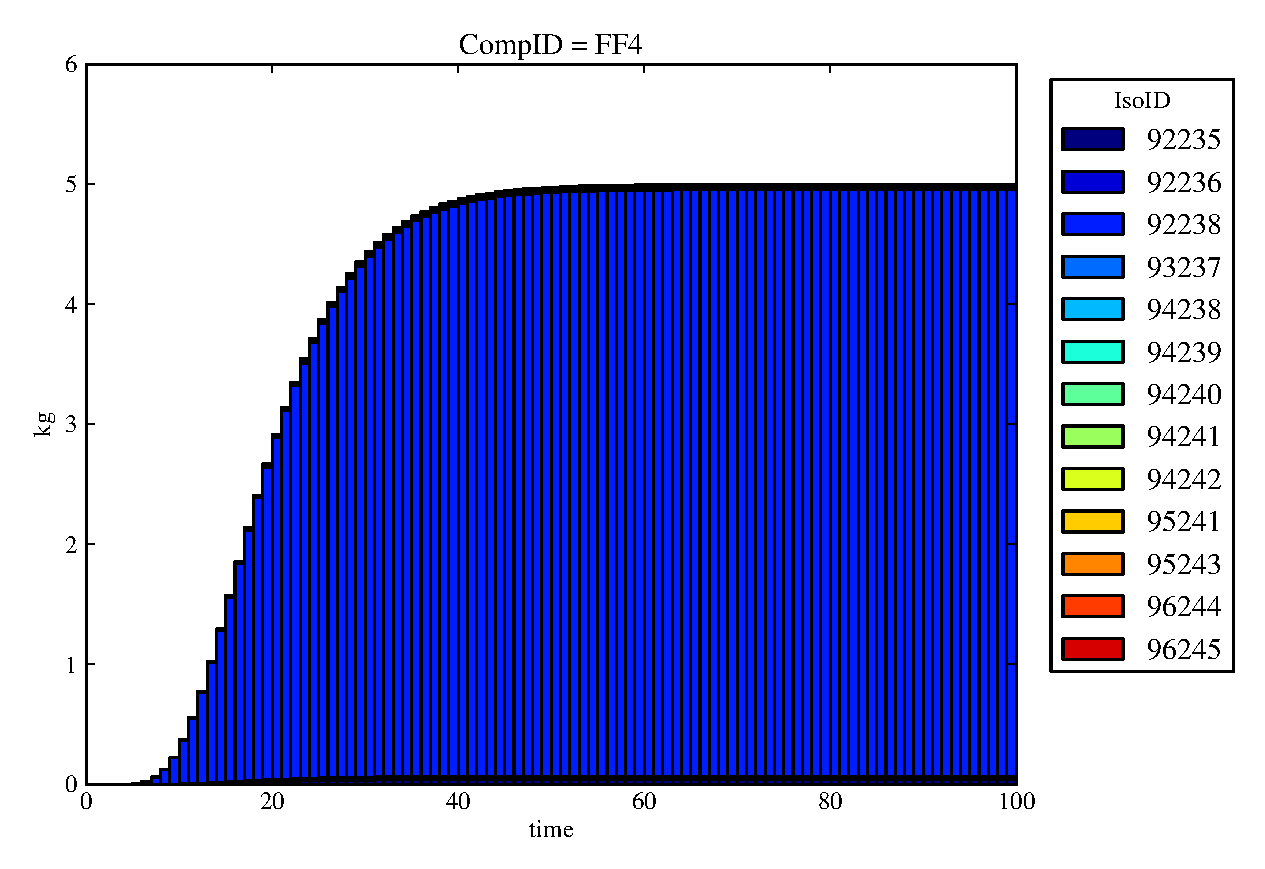
\includegraphics[width=0.6\textwidth]{./results/images/mcIII0.eps}
  \caption[Case MCIII Far Field Contaminants.]{All material is released into
        the Far Field, component 4 (degradation rate $F_d=0.0[y^{-1}]$, reference solubility limit $S_{ref} = 0.001kg/m^3$).}
  \label{fig:mcIII}
\end{figure}



Dual and single parameter verification cases were run to explore the effects of 
sorption and solubility limitation both separately and together.  Results from 
two of these base cases can be found in Figures \ref{fig:mcI} through 
\ref{fig:mcII}.
The fixed maximum transport mode was use between mixed cell components for speed 
and clarity of results.

In the two following simulations, a waste form with 1 kg is introduced to the repository once 
per time step for the first five time steps. Those five waste packages are 
placed into a single buffer component, which is contained by a single far field 
component. All are represented by the Mixed Cell Model. Each component except 
the far field has a degradation rate of 0.1 per time step.


\FloatBarrier

